\documentclass[8pt]{article}
\usepackage[a4paper,landscape,margin=1in]{geometry}
\usepackage{cmbright}
\usepackage{enumitem}
\usepackage{amsmath}
\usepackage{siunitx}
\usepackage{array}
\usepackage{booktabs}
\usepackage{longtable}
\usepackage{xcolor}
\definecolor{urlblue}{HTML}{0000ee}
\usepackage{hyperref}
\hypersetup{%
colorlinks = true,%
urlcolor   = urlblue,%
}
\usepackage{tcolorbox}
\usepackage{varwidth}
\setlength\parindent{0pt}
\pagenumbering{gobble}
\begin{document}
\begin{figure}[!ht]
% MF group logo
\begin{minipage}[b][2.5cm][c]{.72\textwidth}
\href{http://foroozandeh.chem.ox.ac.uk/home}%
{\includegraphics[scale=1.8]{/home/simon/Documents/DPhil/projects/NMR-EsPy/nmrespy/images/mf_logo.png}}
\end{minipage}
% NMR-EsPy logo
\begin{minipage}[b][2.5cm][c]{.27\textwidth}
\href{https://foroozandehgroup.github.io/NMR-EsPy}%
{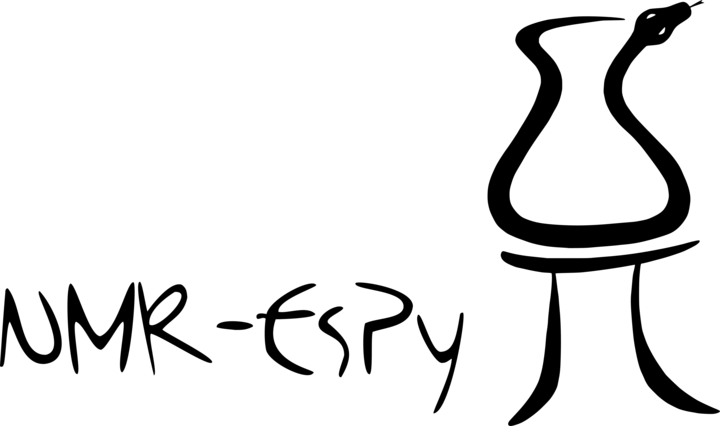
\includegraphics[scale=0.5]{/home/simon/Documents/DPhil/projects/NMR-EsPy/nmrespy/images/nmrespy_full.png}}
\end{minipage}
\end{figure}
\texttt{16:12:57 08-12-23}

Simulated 2,3-Dibromopropanoic acid signal.

\section*{Experiment Information}
\begin{longtable}[l]{c c}
\toprule
Parameter & F1\\
\midrule
Nucleus & \textsuperscript{1}H\\
Transmitter Frequency (MHz) & $\num{500}$\\
Sweep Width (Hz) & $\num{600}$\\
Sweep Width (ppm) & $\num{1.2}$\\
Transmitter Offset (Hz) & $\num{2050}$\\
Transmitter Offset (ppm) & $\num{4.1}$\\
\bottomrule
\end{longtable}

\section*{4.600 - 4.400 ppm}
\begin{longtable}[l]{c c c c c c c}
\toprule
Osc. & $a$ & $\phi$ ($^{\circ}$) & $f ($Hz) & $f ($ppm) & $\eta ($s$^{-1}$) & $\int$\\
\midrule
$\num{1}$ & \begin{tabular}[c]{@{}c@{}}$\num{1.0004}$ \\ $\pm\num{1.3876e-3}$\end{tabular} & \begin{tabular}[c]{@{}c@{}}$\num{8.2802e-2}$ \\ $\pm\num{7.9531e-2}$\end{tabular} & \begin{tabular}[c]{@{}c@{}}$\num{2.2344e+3}$ \\ $\pm\num{2.0361e-3}$\end{tabular} & \begin{tabular}[c]{@{}c@{}}$\num{4.4688}$ \\ $\pm\num{4.0723e-6}$\end{tabular} & \begin{tabular}[c]{@{}c@{}}$\num{6.9995}$ \\ $\pm\num{1.2772e-2}$\end{tabular} & $\num{1.0023}$\\
$\num{2}$ & \begin{tabular}[c]{@{}c@{}}$\num{0.99842}$ \\ $\pm\num{1.4413e-3}$\end{tabular} & \begin{tabular}[c]{@{}c@{}}$\num{2.5957e-2}$ \\ $\pm\num{8.2878e-2}$\end{tabular} & \begin{tabular}[c]{@{}c@{}}$\num{2.243e+3}$ \\ $\pm\num{2.0799e-3}$\end{tabular} & \begin{tabular}[c]{@{}c@{}}$\num{4.486}$ \\ $\pm\num{4.1598e-6}$\end{tabular} & \begin{tabular}[c]{@{}c@{}}$\num{6.9913}$ \\ $\pm\num{1.3017e-2}$\end{tabular} & $\num{1.0005}$\\
$\num{3}$ & \begin{tabular}[c]{@{}c@{}}$\num{1.0002}$ \\ $\pm\num{1.4456e-3}$\end{tabular} & \begin{tabular}[c]{@{}c@{}}$\num{-6.5178e-3}$ \\ $\pm\num{8.2881e-2}$\end{tabular} & \begin{tabular}[c]{@{}c@{}}$\num{2.257e+3}$ \\ $\pm\num{2.0863e-3}$\end{tabular} & \begin{tabular}[c]{@{}c@{}}$\num{4.514}$ \\ $\pm\num{4.1726e-6}$\end{tabular} & \begin{tabular}[c]{@{}c@{}}$\num{7.0169}$ \\ $\pm\num{1.3082e-2}$\end{tabular} & $\num{1.0017}$\\
$\num{4}$ & \begin{tabular}[c]{@{}c@{}}$\num{0.99804}$ \\ $\pm\num{1.3876e-3}$\end{tabular} & \begin{tabular}[c]{@{}c@{}}$\num{4.9217e-2}$ \\ $\pm\num{7.9756e-2}$\end{tabular} & \begin{tabular}[c]{@{}c@{}}$\num{2.2656e+3}$ \\ $\pm\num{2.0404e-3}$\end{tabular} & \begin{tabular}[c]{@{}c@{}}$\num{4.5312}$ \\ $\pm\num{4.0808e-6}$\end{tabular} & \begin{tabular}[c]{@{}c@{}}$\num{6.9955}$ \\ $\pm\num{1.279e-2}$\end{tabular} & $\num{1}$\\
\bottomrule
\end{longtable}

\section*{4.020 - 3.820 ppm}
\begin{longtable}[l]{c c c c c c c}
\toprule
Osc. & $a$ & $\phi$ ($^{\circ}$) & $f ($Hz) & $f ($ppm) & $\eta ($s$^{-1}$) & $\int$\\
\midrule
$\num{1}$ & \begin{tabular}[c]{@{}c@{}}$\num{1.0035}$ \\ $\pm\num{1.2575e-3}$\end{tabular} & \begin{tabular}[c]{@{}c@{}}$\num{-1.1133e-3}$ \\ $\pm\num{7.1748e-2}$\end{tabular} & \begin{tabular}[c]{@{}c@{}}$\num{1.9386e+3}$ \\ $\pm\num{1.9405e-3}$\end{tabular} & \begin{tabular}[c]{@{}c@{}}$\num{3.8772}$ \\ $\pm\num{3.881e-6}$\end{tabular} & \begin{tabular}[c]{@{}c@{}}$\num{7.0167}$ \\ $\pm\num{1.2206e-2}$\end{tabular} & $\num{1.0052}$\\
$\num{2}$ & \begin{tabular}[c]{@{}c@{}}$\num{0.99852}$ \\ $\pm\num{3.8331e-3}$\end{tabular} & \begin{tabular}[c]{@{}c@{}}$\num{-2.1454e-2}$ \\ $\pm\num{0.22074}$\end{tabular} & \begin{tabular}[c]{@{}c@{}}$\num{1.9588e+3}$ \\ $\pm\num{3.6287e-3}$\end{tabular} & \begin{tabular}[c]{@{}c@{}}$\num{3.9176}$ \\ $\pm\num{7.2574e-6}$\end{tabular} & \begin{tabular}[c]{@{}c@{}}$\num{7.0111}$ \\ $\pm\num{2.2801e-2}$\end{tabular} & $\num{1.0003}$\\
$\num{3}$ & \begin{tabular}[c]{@{}c@{}}$\num{1.0026}$ \\ $\pm\num{3.8441e-3}$\end{tabular} & \begin{tabular}[c]{@{}c@{}}$\num{-2.4786e-2}$ \\ $\pm\num{0.21966}$\end{tabular} & \begin{tabular}[c]{@{}c@{}}$\num{1.9612e+3}$ \\ $\pm\num{3.6347e-3}$\end{tabular} & \begin{tabular}[c]{@{}c@{}}$\num{3.9224}$ \\ $\pm\num{7.2695e-6}$\end{tabular} & \begin{tabular}[c]{@{}c@{}}$\num{7.0301}$ \\ $\pm\num{2.2765e-2}$\end{tabular} & $\num{1.004}$\\
$\num{4}$ & \begin{tabular}[c]{@{}c@{}}$\num{1.0009}$ \\ $\pm\num{1.2561e-3}$\end{tabular} & \begin{tabular}[c]{@{}c@{}}$\num{-6.9312e-2}$ \\ $\pm\num{7.1886e-2}$\end{tabular} & \begin{tabular}[c]{@{}c@{}}$\num{1.9814e+3}$ \\ $\pm\num{1.9407e-3}$\end{tabular} & \begin{tabular}[c]{@{}c@{}}$\num{3.9628}$ \\ $\pm\num{3.8815e-6}$\end{tabular} & \begin{tabular}[c]{@{}c@{}}$\num{7.0042}$ \\ $\pm\num{1.2203e-2}$\end{tabular} & $\num{1.0028}$\\
\bottomrule
\end{longtable}

\section*{3.800 - 3.600 ppm}
\begin{longtable}[l]{c c c c c c c}
\toprule
Osc. & $a$ & $\phi$ ($^{\circ}$) & $f ($Hz) & $f ($ppm) & $\eta ($s$^{-1}$) & $\int$\\
\midrule
$\num{1}$ & \begin{tabular}[c]{@{}c@{}}$\num{1.0015}$ \\ $\pm\num{1.3836e-3}$\end{tabular} & \begin{tabular}[c]{@{}c@{}}$\num{6.6528e-2}$ \\ $\pm\num{7.9181e-2}$\end{tabular} & \begin{tabular}[c]{@{}c@{}}$\num{1.8356e+3}$ \\ $\pm\num{2.0225e-3}$\end{tabular} & \begin{tabular}[c]{@{}c@{}}$\num{3.6712}$ \\ $\pm\num{4.045e-6}$\end{tabular} & \begin{tabular}[c]{@{}c@{}}$\num{7.0086}$ \\ $\pm\num{1.2697e-2}$\end{tabular} & $\num{1.0032}$\\
$\num{2}$ & \begin{tabular}[c]{@{}c@{}}$\num{0.99953}$ \\ $\pm\num{1.4671e-3}$\end{tabular} & \begin{tabular}[c]{@{}c@{}}$\num{-6.1993e-3}$ \\ $\pm\num{8.407e-2}$\end{tabular} & \begin{tabular}[c]{@{}c@{}}$\num{1.8442e+3}$ \\ $\pm\num{2.081e-3}$\end{tabular} & \begin{tabular}[c]{@{}c@{}}$\num{3.6884}$ \\ $\pm\num{4.162e-6}$\end{tabular} & \begin{tabular}[c]{@{}c@{}}$\num{6.9937}$ \\ $\pm\num{1.3079e-2}$\end{tabular} & $\num{1.0016}$\\
$\num{3}$ & \begin{tabular}[c]{@{}c@{}}$\num{1.0023}$ \\ $\pm\num{1.4693e-3}$\end{tabular} & \begin{tabular}[c]{@{}c@{}}$\num{5.367e-2}$ \\ $\pm\num{8.412e-2}$\end{tabular} & \begin{tabular}[c]{@{}c@{}}$\num{1.8558e+3}$ \\ $\pm\num{2.0914e-3}$\end{tabular} & \begin{tabular}[c]{@{}c@{}}$\num{3.7116}$ \\ $\pm\num{4.1828e-6}$\end{tabular} & \begin{tabular}[c]{@{}c@{}}$\num{7.0212}$ \\ $\pm\num{1.3102e-2}$\end{tabular} & $\num{1.0038}$\\
$\num{4}$ & \begin{tabular}[c]{@{}c@{}}$\num{0.99981}$ \\ $\pm\num{1.3837e-3}$\end{tabular} & \begin{tabular}[c]{@{}c@{}}$\num{4.9889e-2}$ \\ $\pm\num{7.9332e-2}$\end{tabular} & \begin{tabular}[c]{@{}c@{}}$\num{1.8644e+3}$ \\ $\pm\num{2.0249e-3}$\end{tabular} & \begin{tabular}[c]{@{}c@{}}$\num{3.7288}$ \\ $\pm\num{4.0498e-6}$\end{tabular} & \begin{tabular}[c]{@{}c@{}}$\num{7.0057}$ \\ $\pm\num{1.2713e-2}$\end{tabular} & $\num{1.0016}$\\
\bottomrule
\end{longtable}

\small
\begin{tcolorbox}[hbox]
\begin{varwidth}{12cm}
Estimation performed using \textsc{NMR-EsPy}.\\
Author: Simon Hulse\\
For more information:\\[5pt]
{\raisebox{-4pt}{\includegraphics[scale=0.029]{/home/simon/Documents/DPhil/projects/NMR-EsPy/nmrespy/images/book_icon.png}}}\hspace{1em}\href{https://foroozandehgroup.github.io/NMR-EsPy}{\texttt{https://foroozandehgroup.github.io/NMR-EsPy}}\\[5pt]
{\raisebox{-4pt}{
\includegraphics[scale=0.12]{/home/simon/Documents/DPhil/projects/NMR-EsPy/nmrespy/images/github.png}}}\hspace{1em}\href{https://github.com/foroozandehgroup/NMR-EsPy}{\texttt{https://github.com/foroozandehgroup/NMR-EsPy}}\\[5pt]
{\raisebox{-3pt}{\includegraphics[scale=0.015]{/home/simon/Documents/DPhil/projects/NMR-EsPy/nmrespy/images/email_icon.png}}}\hspace{1em}\href{mailto:simon.hulse@chem.ox.ac.uk?subject=NMR-EsPy query}{\texttt{simon.hulse@chem.ox.ac.uk}}\\[5pt]
If used in a publication, please cite:\\
\begin{itemize}[leftmargin=*, nosep, label={}]
\item Simon G. Hulse, Mohammadali Foroozandeh. \textit{``Newton meets Ockham: Parameter estimation and model selection of NMR data with NMR-EsPy"}. J. Magn. Reson. 338 (2022) 107173.\\ \href{https://doi.org/10.1016/j.jmr.2022.107173}{https://doi.org/10.1016/j.jmr.2022.107173}
\end{itemize}
\end{varwidth}
\end{tcolorbox}
\end{document}